%%%%%%%%%%%%%%%%%%%%%%%%%%%%%%%%%%%%%%%%%%%%%%%%%%%%%%%%%%%%%%%%%%%%%%
\section{Methods}\label{sec:methods}
%%%%%%%%%%%%%%%%%%%%%%%%%%%%%%%%%%%%%%%%%%%%%%%%%%%%%%%%%%%%%%%%%%%%%%

% ==================================================================
\subsection{Overview and notation}\label{subsec:overview}
% ==================================================================
We couple a subnational (municipality-level) reconstruction of Brazil's soy
supply chain with the global FABIO physical multi-regional
input--output (MRIO) framework \cite{bruckner2019fabio}, and attribute the
resulting land-use footprint back to municipalities of origin and forward to
countries of final consumption, annually for 2001--2022 (on the FABIO v2
backend from 2010 and the v1.1 backend before;
Section~\ref{subsubsec:backend}). The construction
proceeds in six stages: (i)~municipal soy accounting, assembling production,
trade and domestic-use quantities for every Brazilian municipality
(Section~\ref{subsec:accounting}); (ii)~livestock-system disaggregation and
feed demand (Section~\ref{subsec:feed}); (iii)~reconciliation of the municipal
totals with national commodity balances (Section~\ref{subsec:balancing});
(iv)~allocation of physical flows between municipalities by cost-minimizing
optimal transport (Section~\ref{subsec:transport}); (v)~linkage of origin
municipalities to importing countries, with re-export disentangling
(Section~\ref{subsec:origin2consumer}); and (vi)~nesting into FABIO
and land-use footprint accounting
(Sections~\ref{subsec:fabio}--\ref{subsec:footprint}). The resulting flows are
validated against the independent Trase supply-chain benchmark and a
pure downscaling baseline (Section~\ref{subsec:validation}). The subnational
tracing framework generalizes the single-year (2013) open model of
Trsek~\cite{trsek2022} to an annual series; a script-level mapping of each
subsection to the released pipeline code is provided with the repository.
Figure~\ref{fig:workflow} summarizes the full pipeline.

\begin{figure}[htbp]
\centering
\begin{tikzpicture}[
  font=\footnotesize,
  stage/.style={draw=black!70, rounded corners=2pt, fill=blue!9,
                text width=51mm, align=center, inner sep=2.2mm},
  data/.style={draw=black!45, densely dashed, fill=black!4,
               text width=28mm, align=center, inner sep=1.6mm},
  res/.style={draw=black!70, thick, rounded corners=2pt, fill=green!10,
              text width=51mm, align=center, inner sep=2.2mm},
  val/.style={draw=black!45, fill=orange!12,
              text width=28mm, align=center, inner sep=1.6mm},
  arr/.style={-{Stealth[length=2.6mm]}, semithick},
  darr/.style={-{Stealth[length=2mm]}, densely dashed, black!55}
]
% --- main pipeline ---
\node[stage] (s1) {\textbf{1~~Municipal soy accounting}~(\S\ref{subsec:accounting})\\
  production, trade and domestic use per municipality and product};
\node[stage, below=4.5mm of s1] (s2) {\textbf{2~~Livestock systems \& feed}~(\S\ref{subsec:feed})\\
  herds split into production systems; municipal soy and cake feed demand};
\node[stage, below=4.5mm of s2] (s3) {\textbf{3~~National balancing}~(\S\ref{subsec:balancing})\\
  municipal totals reconciled with national balances $\rightarrow$
  municipal surpluses and deficits};
\node[stage, below=4.5mm of s3] (s4) {\textbf{4~~Optimal transport}~(\S\ref{subsec:transport})\\
  cost-minimizing inter-municipal flow matrices $\mathbf{F}^{p}$};
\node[stage, below=4.5mm of s4] (s5) {\textbf{5~~Origins $\rightarrow$ importers}~(\S\ref{subsec:origin2consumer})\\
  sourcing matrix; re-export disentangling of bilateral trade};
\node[stage, below=4.5mm of s5] (s6) {\textbf{6~~FABIO nesting \& footprint}~(\S\ref{subsec:fabio}--\ref{subsec:footprint})\\
  municipalities as regions in the global MRIO; EXIOBASE background;
  $\mathbf{H}=\hat{\mathbf{e}}\,\mathbf{L}\,\mathbf{Y}$};
\node[res, below=4.5mm of s6] (out) {\textbf{Result:} hectares of soy land in each origin
  municipality embodied in each country's consumption, annually 2001--2022,
  with biome/frontier attribution};
% --- data inputs (left) ---
\node[data, left=5mm of s1] (d1) {COMEX trade\\ IBGE production, population\\ ABIOVE, ANP, POF};
\node[data, left=5mm of s2] (d2) {IBGE herds\\ GLW3 rasters\\ GLEAM feed rates};
\node[data, left=5mm of s3] (d3) {FAO commodity balance sheets};
\node[data, left=5mm of s5] (d5) {FAOSTAT bilateral trade};
\node[data, left=5mm of s6] (d6) {FABIO v2 / v1.1\\ EXIOBASE 3\\ IBGE soy area};
% --- validation (right) ---
\node[val, right=5mm of s5] (v) {\textbf{Validation}~(\S\ref{subsec:validation})\\
  Trase v2.6.1; downscaling baseline; $r$, RMSE};
% --- arrows ---
\draw[arr] (s1) -- (s2);
\draw[arr] (s2) -- (s3);
\draw[arr] (s3) -- (s4);
\draw[arr] (s4) -- (s5);
\draw[arr] (s5) -- (s6);
\draw[arr] (s6) -- (out);
\draw[darr] (d1) -- (s1);
\draw[darr] (d2) -- (s2);
\draw[darr] (d3) -- (s3);
\draw[darr] (d5) -- (s5);
\draw[darr] (d6) -- (s6);
\draw[darr] (s5) -- (v);
\end{tikzpicture}
\caption{Workflow of the study. Solid boxes are the six model stages
(Sections~\ref{subsec:accounting}--\ref{subsec:footprint}); dashed boxes are
the main data inputs at each stage; the orange box is the independent
validation of the reconstructed flows (Section~\ref{subsec:validation}).
Stages 1--5 reconstruct Brazil's subnational soy supply chain; stage 6 embeds
it in the global FABIO/EXIOBASE input--output framework and computes the
land-use footprint.}\label{fig:workflow}
\end{figure}

\paragraph{Notation.}
Throughout, $m$ and $n$ index Brazil's $\sim$5{,}570 municipalities,
$p\in\{\text{bean},\text{oil},\text{cake}\}$ the three soy products, and
$i,j$ countries. National annual totals from the FAO commodity balance sheet
are written $\CBS{p}{\text{use}}$, e.g.\ $\CBS{\text{oil}}{\text{food}}$
for the national food use of soy oil. Matrices and vectors are set in bold,
$\diag(\cdot)$ denotes a diagonal matrix and $\mathbf{I}$ the identity; a hat
($\hat{\mathbf{e}}$) diagonalizes a vector.

\paragraph{The mass-conserving allocation operator.}
A single operation recurs throughout the subnational reconstruction: a
national total $T$ is distributed across municipalities in proportion to an
observable weight $w_m$,
\begin{equation}\label{eq:split}
  q_m \;=\; \frac{w_m}{\sum_{n}w_{n}}\;T,
  \qquad\text{so that}\qquad \sum_m q_m = T .
\end{equation}
The stages below differ mainly in the choice of weight $w_m$; the released
pipeline checks each allocation against its national total at run time and
halts on any violation. Table~\ref{tab:weights}
collects the weights used for the domestic-use items.

% ==================================================================
\subsection{Municipal soy accounting}\label{subsec:accounting}
% ==================================================================
% Pipeline step 00 (00_data_preparation) and step 01.

\subsubsection{Municipal supply, trade and infrastructure}\label{subsubsec:assemble}
Municipality-level exports and imports of the three soy products are read from COMEX customs records, aggregated from monthly to annual tonnages and matched to IBGE municipality identifiers. Exports declared without a municipality of origin are redistributed across the declared exporters of the same product and destination in proportion to their declared volumes, thereby conserving national totals. Undeclared imports are negligible and are not redistributed. Installed crushing and refining capacity (ABIOVE) is divided equally among each state's active plants and summed per municipality. Grain storage capacity is aggregated from georeferenced warehouse records, and biodiesel capacity (ANP) is attributed to soy according to the soy feedstock share of each macro-region. All geometries are projected onto a national planar reference system (SIRGAS~2000 / Brazil Polyconic, EPSG:5880) and each municipality is represented by its administrative centre. Straight-line distances between administrative centres are used to calculate transport costs in Section~\ref{subsec:transport}.

\subsubsection{Domestic-use estimation}\label{subsubsec:domuse}

Every item intended for domestic use in the national commodity balance is distributed across municipalities using the allocation operator (see equation \eqref{eq:split}) and the weights in Table~\ref{tab:weights}. The national soybean crush is allocated in proportion to crushing capacity. Municipal oil and cake output then follow from the crush, with conversion yields derived each year from the national balance itself (the ratio of national oil and cake production to beans crushed is approximately 20\% oil and 75\% cake, with a 5\% processing loss, consistent with values in the literature). The food use of beans and oil is allocated by household soy oil consumption, which is calculated as the state-level per capita acquisition rate (POF) multiplied by the municipal population. Other uses, such as biodiesel production, are allocated according to soy-attributable biodiesel capacity. Seed use is allocated according to soybean production, and stock changes are allocated according to storage capacity for beans and to municipal oil and cake production for the processed products. A net national stock addition is carried on the use side, whereas a net national withdrawal is treated as a supply component (see Eq.~\ref{eq:balance}) and distributed across municipalities by those same stock weights, but added to municipal supply rather than subtracted from use. This mirrors the commodity-balance identity in which a drawdown is a genuine source of current-year supply and ensures that every municipal use remains non-negative, as required by the re-export inversion in Section ~\ref{subsubsec:reexport}. A storage-based split of a drawdown on the use side would instead result in the net use of high-storage, low-use municipalities being negative.

\begin{table}[htbp]
\small
\caption{Domestic-use items as instances of the allocation operator
\eqref{eq:split}: each item is a national commodity-balance total distributed
across municipalities by the stated weight $w_m$.}\label{tab:weights}
\begin{tabular}{@{}ll@{}}
\toprule
Use item & Allocation weight $w_m$ \\
\midrule
Processing (crush)  & installed crushing capacity \\
Food (beans, oil)   & per-capita soy-oil acquisition $\times$ population \\
Other (biodiesel)   & soy-attributable biodiesel capacity \\
Seed                & soybean production \\
Stock change        & storage capacity (beans), production (oil, cake); addition $\to$ use, withdrawal $\to$ supply \\
\botrule
\end{tabular}
\end{table}

% ==================================================================
\subsection{Livestock systems and feed demand}\label{subsec:feed}
% ==================================================================
% Pipeline steps 02-03.
As soy feed intake varies significantly across production systems, IBGE municipal herd counts are divided into the following categories: extensive and intensive chickens; extensive, intensive and industrial pigs; and grassland- and mixed-based cattle and buffalo, with each category divided into dairy and meat. System shares are obtained using area-weighted zonal statistics of the 2010 FAO gridded livestock rasters (GLW3) and the GLEAM ruminant production system map for each municipality. Where a municipality reports a herd but had no gridded animals in 2010, the state mean share is used. Dairy herds are identified by milked cow counts and feedlot cattle, which are only reported in the agricultural census, are extrapolated from 2006 using the national confinement growth rate while holding the municipal pattern fixed. The full split formulas are given in Appendix ~\ref{app:livestock}. Each species' subsystems are verified to partition its reported herd exactly.

Feed demand is calculated by multiplying each herd by its GLEAM per-animal intake, i.e. annual dry-matter intake multiplied by the proportion sourced from soybeans and soy cake, converted to as-fed tonnes at 88\% dry matter content. One national factor per product then rescales the resulting bottom-up totals to the FAO national feed figures (an application of equation \eqref{eq:split} with the bottom-up municipality$\times$system feed matrix as weight), preserving the spatial and cross-system distribution while matching the national constraint. Municipal feed demand for beans and cake is the sum over systems. Holding the 2010 system shares constant over the study period is a simplification: herd sizes remain annual, misclassification affects only how a municipality's herd is split across intake intensities, and the subsequent rescaling of all bottom-up feed to the national FAO totals bounds the aggregate error. The residual uncertainty grows with distance from the 2010 reference year. Figure~\ref{fig:feed} sketches the construction.

\begin{figure}[htbp]
\centering
\begin{tikzpicture}[font=\footnotesize,
  box/.style={draw=black!60, rounded corners=2pt, fill=blue!6,
              text width=27mm, align=center, inner sep=1.8mm},
  arr/.style={-{Stealth[length=2.4mm]}, semithick}]
% --- raster with municipality polygon ---
\begin{scope}
\foreach \i/\j/\c in {0/0/10, 1/0/25, 2/0/45, 3/0/15,
                      0/1/30, 1/1/55, 2/1/70, 3/1/35,
                      0/2/20, 1/2/60, 2/2/40, 3/2/10,
                      0/3/5,  1/3/30, 2/3/20, 3/3/8}
  \fill[orange!\c] (\i*0.45,\j*0.45) rectangle (\i*0.45+0.45,\j*0.45+0.45);
\draw[black!30, step=0.45cm] (0,0) grid (1.8,1.8);
\draw[black!80, thick] (0.35,0.15) -- (1.5,0.35) -- (1.7,1.2)
  -- (1.0,1.7) -- (0.2,1.3) -- cycle;
\end{scope}
\node[below, text width=32mm, align=center] at (0.9,-0.2)
  {2010 gridded livestock (GLW3, GLEAM) $\cap$ municipality $m$};
\draw[arr] (2.15,0.9) -- (3.15,0.9);
% --- system-share bar ---
\begin{scope}[xshift=3.5cm]
\fill[orange!25] (0,0) rectangle (0.5,0.95);
\fill[orange!55] (0,0.95) rectangle (0.5,1.5);
\fill[orange!90] (0,1.5) rectangle (0.5,1.8);
\draw[black!70] (0,0) rectangle (0.5,1.8);
\node[right, font=\tiny] at (0.52,0.5)  {extensive};
\node[right, font=\tiny] at (0.52,1.22) {intensive};
\node[right, font=\tiny] at (0.52,1.65) {industrial};
\node[below, text width=24mm, align=center] at (0.8,-0.2)
  {production-system shares of $m$};
\end{scope}
\draw[arr] (5.9,0.9) -- (6.9,0.9);
% --- herd box ---
\node[box, anchor=west] (herd) at (7.0,0.9)
  {annual IBGE herd of $m$, split by the 2010 system shares};
% --- second row ---
\node[box, below=18mm of herd] (intake)
  {$\times$ GLEAM per-animal soybean and soy-cake intake of each system};
\node[box, fill=green!10, left=12mm of intake] (feed)
  {municipal feed demand for beans and cake, rescaled to the FAO national
   feed totals~\eqref{eq:split}};
\draw[arr] (herd) -- (intake);
\draw[arr] (intake) -- (feed);
\end{tikzpicture}
\caption{From herds to municipal soy feed demand. Municipal herd counts
(annual) are split into production systems using the shares implied by the
2010 gridded-livestock rasters within each municipality; each system's herd
is multiplied by its per-animal soy and soy-cake intake, and the bottom-up
totals are rescaled to match the national feed use reported by
FAO.}\label{fig:feed}
\end{figure}

% ==================================================================
\subsection{National balancing and trade reconciliation}\label{subsec:balancing}
% ==================================================================
% Pipeline steps 04-05.
For each product, the national commodity balance imposes the supply--use
identity
\begin{equation}\label{eq:balance}
\begin{aligned}
  \underbrace{\text{production}+\text{imports}+\text{stock withdrawal}}_{\text{supply}}
  \hspace{28mm}&\\[-1pt]
  =\;\underbrace{\text{exports}+\text{food}+\text{feed}+\text{seed}
    +\text{processing}+\text{other}}_{\text{use}}&\,.
\end{aligned}
\end{equation}
First, municipal exports and imports are harmonised with the FABIO/FAOSTAT bilateral trade classification. Destinations absent from the bilateral trade list are collapsed into a rest-of-world aggregate. This step aligns classifications and applies no rescaling. Any remaining supply-use residual at the national level is absorbed into the stock term and each balance item is then proportionally rescaled by equation \eqref{eq:split} using the item's municipal distribution as the weight. This ensures that every municipal aggregate matches its national total exactly. Consistent with the supply-use identity (Equation \eqref{eq:balance}), a net national stock withdrawal is carried out on the supply side: the drawdown is distributed across municipalities by the stock weights (storage capacity for beans and production for oil and cake) and added to municipal supply. This ensures that every municipal use remains non-negative (additional years are unchanged and carried on the use side). As the model is a single annual snapshot, tonnes supplied from a drawdown, which were physically grown in earlier years, inherit the current year's soy-area intensity
(Section~\ref{subsec:footprint}). This approximation only affects the small share of throughput met from net stock changes. Finally, each municipality's product balance defines its surplus or deficit:
\begin{equation}\label{eq:surplus}
  \text{surplus}^p_m=\max\!\big(\text{supply}^p_m-\text{use}^p_m,\,0\big),
  \qquad
  \text{deficit}^p_m=\max\!\big(\text{use}^p_m-\text{supply}^p_m,\,0\big),
\end{equation}
These then determine the inter-municipal flows of Section~\ref{subsec:transport}.
The positive-part decomposition is lossless: surplus minus deficit equals the
signed net position of every municipality, and the two totals match by
construction after the above rescaling, as required by the balanced transportation problem. At the national level, the corresponding residual cannot be resolved into flows. There, it is retained as Fabio's signed balancing column, which re-enters the model as a dedicated final-demand category (see Sections~\ref{subsubsec:mrsut} and~\ref{subsubsec:stressor}).

% ==================================================================
\subsection{Subnational transport allocation}\label{subsec:transport}
% ==================================================================
% Pipeline step 07 (07_transport_R.R). The multimodal GAMS/LP variant
% (steps 06/07_GAMS, transport_lp/) is intentionally not described here.
Municipal surpluses and deficits are connected by \emph{cost-minimizing
optimal transport} rather than a gravity or distance-decay model, on the
premise that bulk-commodity logistics minimize freight cost and that freight
cost increases with distance. The cost metric is the straight-line distance
between municipal seats, which requires no network parameters that would be
unobservable for parts of the study period; its adequacy is tested against
the independent benchmark
(Section~\ref{subsec:validation}). The multimodal network data (roads, rail,
waterways, ports; Data) support an experimental cost-based variant that is
carried in the repository but not used for the reported results.
\textcolor{red}{\textbf{[ADD MULTIMODAL VARIANT: describe the multimodal
cost-based transport model here once it is runnable, and report the
sensitivity of the footprints to the cost metric.]}} For each
product $p$, the inter-municipal flow matrix $\mathbf{F}^p$ solves the
balanced transportation problem
\begin{equation}\label{eq:ot}
  \mathbf{F}^{p}=\argmin_{\mathbf{F}\ge0}\ \sum_{m,n}F_{mn}\,d_{mn}
  \quad\text{s.t.}\quad
  \sum_{n}F_{mn}=\text{surplus}^p_m,\ \
  \sum_{m}F_{mn}=\text{deficit}^p_n,
\end{equation}
where $d_{mn}$ is the straight-line distance between the seats of
municipalities $m$ and $n$ (the two margins are balanced beforehand by
proportionally scaling the larger one). The problem is solved exactly by the
network-simplex algorithm (R package \texttt{transport}
\cite{schuhmacher2023transport}), separately for beans, oil and cake. The
solution is a deterministic, mass-conserving flow matrix whose margins
reproduce the municipal surpluses and deficits by construction.
Figure~\ref{fig:transport} contrasts this allocation with the
pure-downscaling baseline used for validation
(Section~\ref{subsubsec:benchmarks}) on a stylized example.

\begin{figure}[htbp]
\centering
\begin{tikzpicture}[font=\footnotesize,
  sur/.style={circle, fill=green!45, draw=black!60, inner sep=0pt},
  def/.style={circle, fill=orange!55, draw=black!60, inner sep=0pt},
  off/.style={circle, fill=black!10, draw=black!40, inner sep=0pt},
  arr/.style={-{Stealth[length=2.4mm]}, semithick},
  dist/.style={densely dotted, black!60},
  lab/.style={font=\tiny},
  note/.style={align=left, anchor=north west, font=\tiny, text width=48mm}]
% same stylized state and the same four municipal seats in both panels
\def\stateoutline{\draw[black!40, fill=black!2]
  plot [smooth cycle, tension=0.7] coordinates
  {(0.5,1.0) (1.5,-0.1) (3.7,-0.4) (5.2,0.7) (5.1,2.7) (3.3,3.5) (1.0,3.1)};}
% ================= panel a: optimal transport =================
\begin{scope}
\node[font=\footnotesize\bfseries, anchor=west] at (-0.2,3.9)
  {a~~subnational model: cost-minimizing optimal transport \eqref{eq:ot}};
\stateoutline
% municipal seats: circle area ~ tonnage
\node[sur, minimum size=6.3mm] (m1) at (1.2,2.6) {};
\node[sur, minimum size=4.5mm] (m2) at (1.4,0.7) {};
\node[def, minimum size=6.9mm] (n1) at (4.3,2.4) {};
\node[def, minimum size=3.5mm] (n2) at (4.1,0.5) {};
\node[above=0.6mm of m1, lab] {$m_1$: $+100$\,t};
\node[below=0.6mm of m2, lab] {$m_2$: $+50$\,t};
\node[above=0.6mm of n1, lab] {$n_1$: $-120$\,t};
\node[below=0.6mm of n2, lab] {$n_2$: $-30$\,t};
\node[below=0.5mm of n1, lab, text=black!60] {(e.g.\ a port)};
% the unused pair: distances are defined between every pair of seats
\draw[dist] (m1) -- node[sloped, below, lab, pos=0.76] {$d_{m_1n_2}$} (n2);
% cost-minimizing flows (labels kept away from the central crossing)
\draw[arr] (m1) -- node[sloped, above, lab, pos=0.45] {$F_{m_1n_1}=100$\,t} (n1);
\draw[arr] (m2) -- node[sloped, above, lab, pos=0.58] {$20$\,t} (n1);
\draw[arr] (m2) -- node[sloped, above, lab, pos=0.45] {$30$\,t} (n2);
% right-hand annotation column
\node[note] at (6.1,3.5)
  {seats $=$ administrative centres\\
   (planar projection, EPSG:5880)\\[3pt]
   $d_{mn}$: straight line between the\\
   seats of \emph{every} pair; dotted:\\
   an unused pair\\[3pt]
   arrows: the flow matrix $\mathbf{F}$,\\
   the cheapest assignment that\\
   clears every surplus (green)\\
   and deficit (orange)\\[3pt]
   the margins \eqref{eq:surplus} already\\
   contain trade: imports add to a\\
   seat's supply, exports (e.g.\ at\\
   ports) to its use};
\end{scope}
% ================= panel b: downscaling baseline =================
\begin{scope}[yshift=-6.0cm]
\node[font=\footnotesize\bfseries, anchor=west] at (-0.2,3.9)
  {b~~downscaling baseline: production shares only \eqref{eq:split}};
\stateoutline
% same seats; the domestic network is ignored (gray)
\node[sur, minimum size=6.3mm] (p1) at (1.2,2.6) {};
\node[sur, minimum size=4.5mm] (p2) at (1.4,0.7) {};
\node[off, minimum size=3.5mm] (q1) at (4.3,2.4) {};
\node[off, minimum size=3.0mm] (q2) at (4.1,0.5) {};
\node[above=0.6mm of p1, lab] {$m_1$: $\tfrac{2}{3}$ of production};
\node[below=0.6mm of p2, lab] {$m_2$: $\tfrac{1}{3}$ of production};
% destination box, aligned with the annotation column of panel a
\node[draw=black!60, rounded corners=2pt, fill=black!5, align=center,
      inner sep=1.8mm, text width=24mm] (dest) at (7.4,1.5)
  {country $j$\\ imports 100\,t};
% exports split by production share; no distances involved
\draw[arr] (p1) -- node[sloped, above, lab, pos=0.45] {$67$\,t} (dest.168);
\draw[arr] (p2) -- node[sloped, above, lab, pos=0.45] {$33$\,t} (dest.192);
\node[note] at (6.1,0.5)
  {no distances, no inter-municipal\\
   flows: bilateral exports are split\\
   $\propto$ production share; deficits\\
   and ports (gray) play no role};
\end{scope}
\end{tikzpicture}
\caption{Two ways of attributing trade to origin municipalities, on the same
stylized geography.
\textbf{a}, The subnational model: each municipality is represented by its
administrative centre (seat), and $d_{mn}$ is the straight-line (Euclidean)
distance between the seats of every pair of municipalities in the planar
national projection. The flow matrix $\mathbf{F}$ (arrows) is the solution
of the balanced transportation problem \eqref{eq:ot} --- the cheapest
mass-conserving assignment of surpluses (green, circle area proportional to
tonnage) to deficits (orange): here $m_2$ serves the nearby small deficit
$n_2$ and the remainder flows to $n_1$; the pair $m_1n_2$ (dotted) is priced
but not used. International trade is embedded in
the margins (Eqs.~\ref{eq:balance} and~\ref{eq:surplus}): a municipality's
imports add to its supply and its exports add to its use, so an exporting
port municipality appears simply as a large deficit ($n_1$) that attracts
inter-municipal flows --- no separate trade arrows are needed.
\textbf{b}, The pure-downscaling
baseline used for validation (Section~\ref{subsubsec:benchmarks}) ignores
the domestic network entirely: exports to each destination are split across
municipalities in proportion to their production share (here
$\tfrac{2}{3}\times100=67$\,t and $33$\,t), i.e.\ the allocation
operator \eqref{eq:split} applied directly to bilateral exports; deficits,
ports and inter-municipal flows (gray) play no role.}\label{fig:transport}
\end{figure}


% ==================================================================
\subsection{From origins to consumers}\label{subsec:origin2consumer}
% ==================================================================
% Pipeline steps 08 and 12.

\subsubsection{Linking origin municipalities to importing countries}\label{subsubsec:exportlink}
Customs data attach two labels to every exported tonne: the municipality
that shipped it and the country that first imported it. Neither is the label
the footprint needs, which is the municipality that grew the soy and the
country that finally consumes it. This section corrects both, first
backwards within Brazil (this part), then forwards across borders
(Section~\ref{subsubsec:reexport}).

The transport flows of Section~\ref{subsec:transport} are the tracing
device, after one completion: they record only what moves between
municipalities, so the part of each municipality's supply that stays and is
used at home is added on the diagonal,
\begin{equation}\label{eq:augment}
  \tilde F^p_{mn} \;=\; F^p_{mn} \;+\;
  \mathbf{1}[m=n]\,\big(\text{supply}^p_m-\text{surplus}^p_m\big),
\end{equation}
so that every tonne a municipality handles is accounted for, whether it
travelled or stayed: the rows of $\tilde{\mathbf{F}}^p$ sum to total
municipal supply, its columns to total municipal use.
Figure~\ref{fig:augment} illustrates the construction and the sourcing
shares derived from it.

\begin{figure}[htbp]
\centering
\begin{tikzpicture}[font=\footnotesize,
  lab/.style={font=\tiny, align=center},
  note/.style={font=\tiny, align=left, anchor=west},
  arr/.style={-{Stealth[length=2.2mm]}, semithick}]
% ================= panel a: the augmented matrix =================
\node[font=\footnotesize\bfseries, anchor=west] at (-0.6,3.55)
  {a~~the augmented flow matrix $\tilde{\mathbf{F}}^p$ \eqref{eq:augment}};
% cell size 0.55; row m from top, column n from left
\fill[black!3] (0,0) rectangle (2.75,2.75);
% inter-municipal flows F (blue, off-diagonal)
\fill[blue!22] (1.65,2.20) rectangle (2.20,2.75);  % m1 -> n4
\fill[blue!45] (1.65,1.65) rectangle (2.20,2.20);  % m2 -> n4
\fill[blue!28] (0.00,1.65) rectangle (0.55,2.20);  % m2 -> n1
\fill[blue!16] (1.10,2.20) rectangle (1.65,2.75);  % m1 -> n3
\fill[blue!20] (2.20,1.10) rectangle (2.75,1.65);  % m3 -> n5
\fill[blue!14] (0.55,0.00) rectangle (1.10,0.55);  % m5 -> n2
% retained own supply (green, diagonal)
\foreach \k in {0,...,4}
  \fill[green!40] (\k*0.55,2.75-\k*0.55-0.55) rectangle (\k*0.55+0.55,2.75-\k*0.55);
% grid + highlighted column n4
\draw[black!30, step=0.55] (0,0) grid (2.75,2.75);
\draw[black!80, thick] (1.65,0) rectangle (2.20,2.75);
% axis labels + matrix symbol
\node[font=\footnotesize, anchor=south east] at (-0.30,2.80) {$\tilde{\mathbf{F}}^p$};
\node[lab, anchor=south] at (1.375,2.87) {destination municipality $n$};
\node[lab, anchor=south, rotate=90] at (-0.22,1.375) {origin municipality $m$};
% annotation column, evenly spaced
\node[note, text width=42mm] at (4.30,2.40)
  {\textcolor{blue!60!black}{off-diagonal}: inter-municipal flows
   $\mathbf{F}^p$ (\S\ref{subsec:transport})};
\draw[arr, black!55] (4.22,2.40) -- (1.95,2.47);
\node[note, text width=42mm] at (4.30,1.40)
  {\textcolor{green!45!black}{diagonal}: retained own supply\\
   $=$ supply $-$ surplus};
\draw[arr, black!55] (4.22,1.40) -- (1.44,1.38);
\node[note, text width=42mm] at (4.30,0.40)
  {rows sum to total supply of $m$;\\ columns to total use of $n$};
% ================= panel b: column -> shares -> exports =================
\begin{scope}[yshift=-4.3cm]
\node[font=\footnotesize\bfseries, anchor=west] at (-0.6,2.75)
  {b~~from one destination column to origin-resolved exports};
% --- bar 1: the framed column, origin labels on the left ---
\fill[blue!22]  (0,1.50) rectangle (0.55,2.05);
\fill[blue!45]  (0,0.65) rectangle (0.55,1.50);
\fill[green!40] (0,0.00) rectangle (0.55,0.65);
\draw[black!70] (0,0) rectangle (0.55,2.05);
\node[lab, anchor=east] at (-0.10,1.775) {from $m_1$};
\node[lab, anchor=east] at (-0.10,1.075) {from $m_2$};
\node[lab, anchor=east] at (-0.10,0.325) {own supply};
\node[lab, anchor=north, text width=18mm] at (0.275,-0.18) {column $n$ of $\tilde{\mathbf{F}}^p$};
% --- arrow 1 ---
\draw[arr] (0.90,1.02) -- node[lab, above=0.6mm] {$\div$ column sum} (2.70,1.02);
% --- bar 2: the shares, phi values on the right ---
\begin{scope}[xshift=3.0cm]
\fill[blue!22]  (0,1.50) rectangle (0.55,2.05);
\fill[blue!45]  (0,0.65) rectangle (0.55,1.50);
\fill[green!40] (0,0.00) rectangle (0.55,0.65);
\draw[black!70] (0,0) rectangle (0.55,2.05);
\node[lab, anchor=west] at (0.65,1.775) {$\phi_{m_1n}=0.27$};
\node[lab, anchor=west] at (0.65,1.075) {$\phi_{m_2n}=0.41$};
\node[lab, anchor=west] at (0.65,0.325) {$\phi_{nn}=0.32$};
\node[lab, anchor=north, text width=22mm] at (0.55,-0.18) {sourcing shares of $n$, sum $=1$};
\end{scope}
% --- arrow 2 ---
\draw[arr] (5.35,1.02) -- node[lab, above=0.6mm] {$\times\ E^p_{nj},\ \delta^p_m$} (7.05,1.02);
% --- result box ---
\node[draw=black!60, rounded corners=2pt, fill=black!5, align=center,
      inner sep=1.8mm, text width=31mm, anchor=west] at (7.25,1.02)
  {exports of $n$ attributed\\ to origin municipalities:\\
   $X^p_{mj}$ \eqref{eq:src2exp}};
\end{scope}
\end{tikzpicture}
\caption{Completing the flow matrix and reading off sourcing shares.
\textbf{a}, The inter-municipal flows $\mathbf{F}^p$ of
Section~\ref{subsec:transport} occupy the off-diagonal (blue); the diagonal
(green) adds each municipality's retained own supply \eqref{eq:augment}, so
rows sum to total municipal supply and columns to total municipal use.
\textbf{b}, One destination column (framed in \textbf{a}), divided by its
sum, gives the sourcing shares $\phi^p_{mn}$: the composition of
municipality $n$'s use by origin, including $n$'s own retained supply.
Weighting $n$'s observed exports $E^p_{nj}$ by these shares and by the
domestic-origin share $\delta^p_m$ yields the origin-resolved exports
$X^p_{mj}$ of Eq.~\eqref{eq:src2exp}.}\label{fig:augment}
\end{figure}


Every exported tonne is then unwound to its origin,
\begin{equation}\label{eq:src2exp}
  X^p_{mj}=\delta^p_m\sum_{n}\phi^p_{mn}\,E^p_{nj},
\end{equation}
where $E^p_{nj}$ are the observed exports of municipality $n$ to country
$j$; the sourcing share
$\phi^p_{mn}=\tilde F^p_{mn}/\sum_{m'}\tilde F^p_{m'n}$ is the fraction
of $n$'s total use that originated in municipality $m$ (including $m=n$);
and the domestic-origin share
$\delta^p_m=(\text{supply}^p_m-\text{imports}^p_m)/\text{supply}^p_m$
strips out quantities of foreign origin (withdrawal-supplied tonnes count as
domestic under the supply-side stock treatment;
Section~\ref{subsubsec:domuse}).
Local consumption is traced with the same formula through a synthetic
domestic column added to the export table (for beans net of the crush, which
is traced through the oil and cake chains instead), and oil and cake are
traced one step further back, to the bean-growing municipalities, by
premultiplying their origin-to-destination matrices with the bean sourcing
shares and the bean domestic-origin share.

\subsubsection{Re-export disentangling}\label{subsubsec:reexport}
To attribute internationally traded soy to its true origin, bilateral trade is
disentangled with a Leontief-type inversion. For each commodity, let
$\mathbf{T}$ be the bilateral trade matrix, with Brazil replaced by its
municipalities for the soy products, and $\mathbf{u}$ the vector of total
use by region. Normalizing trade by destination use and summing the infinite
re-export chain,
\begin{equation}\label{eq:reex}
  \mathbf{R}=\mathbf{T}\,\hat{\mathbf{u}}^{-1},
  \qquad
  \mathbf{L}_{\mathrm{trade}}=(\mathbf{I}-\mathbf{R})^{-1}
  =\sum_{k=0}^{\infty}\mathbf{R}^{k},
\end{equation}
where the entry $R_{ij}$ is the share of region $j$'s total use supplied by
imports from region $i$, so that $\mathbf{R}^{k}$ carries the flows that
have been re-exported $k$ times and the inverse sums chains of every length.
Retaining only the quantities produced domestically (via each region's domestic supply share), scaled by each destination's domestic use, yields the origin-to-consumption matrix. The entry in this matrix gives the quantity produced in region (or municipality) $i$ and ultimately consumed in region $j$. The inversion
assumes proportional mixing of domestic production and imports within each
region's use, the standard assumption of physical trade-linkage accounting \cite{kastner2011tracing}.
At the municipal level, this is stronger than at the country level in an MRIO, since it also governs which producing municipalities supply each destination. The export leg is nonetheless observed at the municipality–country level, so destination differences that operate through port choice are retained, and the assumption binds only to sourcing within a port's hinterland and to the international re-export chain. Origin-specific contracting (e.g.\ the Amazon
Soy Moratorium and certified zero-deforestation chains) is not resolved; its
bias is bounded in Section~\ref{subsubsec:uncertainty}.
Its row and column sums recover each region's domestic supply and use.
\footnote{For soy products, the regional dimension comprises non-Brazilian trading countries and Brazilian municipalities, with Brazil as a whole fully replaced by its municipalities. This replacement is enforced throughout the processing of the trade data so that no national Brazilian record re-enters the inversion.} The inversion is computed exactly by a sparse solver. If the sparse factorisation fails numerically, a dense solve is attempted. Only as a last resort is a small diagonal ridge applied to lift a genuine unit
eigenvalue of $\mathbf{R}$ (which arises when a commodity's recorded global
trade is entirely re-exported). The years in which the ridge is required are
documented with the released code. Figure~\ref{fig:reexport} illustrates the correction for a
stylized example.

\begin{figure}[htbp]
\centering
\begin{tikzpicture}[font=\footnotesize,
  cty/.style={draw=black!60, rounded corners=2pt, fill=black!5,
              minimum width=19mm, minimum height=7mm, align=center},
  mun/.style={draw=black!70, rounded corners=2pt, fill=green!12,
              minimum width=19mm, minimum height=7mm, align=center},
  arr/.style={-{Stealth[length=2.4mm]}, semithick}]
% --- observed trade ---
\node[font=\footnotesize\bfseries, anchor=west] at (-0.4,1.5)
  {a~~observed trade: country of \emph{first import}};
\node[mun] (m1) at (0.8,0) {municipality $m$};
\node[cty] (nl1) at (4.7,0) {Netherlands};
\node[cty] (de1) at (8.6,0) {Germany};
\draw[arr] (m1) -- node[above]{100\,t} (nl1);
\draw[arr] (nl1) -- node[above]{80\,t re-exported} (de1);
\node[below=0.5mm of nl1, font=\tiny, text=black!70] {consumes 20\,t};
\node[below=0.5mm of de1, font=\tiny, text=black!70] {consumes 80\,t};
% --- after inversion ---
\node[font=\footnotesize\bfseries, anchor=west] at (-0.4,-1.9)
  {b~~after re-export disentangling \eqref{eq:reex}: country of \emph{consumption}};
\node[mun] (m2) at (0.8,-3.3) {municipality $m$};
\node[cty] (nl2) at (4.7,-3.3) {Netherlands};
\node[cty] (de2) at (8.6,-3.3) {Germany};
\draw[arr] (m2) -- node[above]{20\,t} (nl2);
\draw[arr] (m2.south) .. controls (2.6,-4.6) and (6.6,-4.6) ..
  node[below]{80\,t} (de2.south);
\end{tikzpicture}
\caption{Re-export disentangling. \textbf{a}, Customs records attribute all
100\,t exported by municipality $m$ to the Netherlands, the country of first
import, although 80\,t are re-exported and consumed in Germany.
\textbf{b}, The trade inversion \eqref{eq:reex} sums re-export chains of any
length and reattributes each tonne to its country of final consumption,
leaving only the 20\,t actually consumed in the Netherlands attributed
there.}\label{fig:reexport}
\end{figure}

% ==================================================================
\subsection{Nesting into FABIO}\label{subsec:fabio}
% ==================================================================
% Pipeline steps 13-19.
The reconstructed municipal soy flows are embedded in the FABIO~v2
physical MRIO, in which a \emph{process} is a region$\times$commodity unit.
Brazil's national soy commodities and processes are removed and replaced by
their municipal counterparts throughout, so that municipalities enter the
global model as additional regions. Figure~\ref{fig:nesting} illustrates the
nesting and the role of the Leontief inverses used below.

\begin{figure}[htbp]
\centering
% --- panel a: how municipal Brazil is inserted into the FABIO process list ---
\begin{tikzpicture}[font=\footnotesize,
  arr/.style={-{Stealth[length=2.4mm]}, semithick},
  brc/.style={decorate, decoration={brace, amplitude=3pt}, black!60},
  dimlab/.style={font=\tiny, black!70, align=left}]
\node[font=\footnotesize\bfseries] at (-2.2,4.95) {a};
% ---- left column: original FABIO process list ----
\draw[fill=black!6, draw=black!70] (0,0) rectangle (2.9,4.6);
\fill[blue!15] (0,1.7) rectangle (2.9,2.9);
\fill[blue!70] (0,2.24) rectangle (2.9,2.44); % national soy stripe
\draw[black!70] (0,1.7) rectangle (2.9,2.9);
\node[font=\tiny, align=center] at (1.45,3.85)
  {180 other regions $\times$ 123 items\\ $=$ 22{,}140 processes};
\node[font=\tiny] at (1.45,1.95) {Brazil: 123 items};
\node[font=\tiny] at (1.45,0.8) {\vdots};
\node[font=\tiny, anchor=east, align=right, text width=15mm] at (-0.15,2.34)
  {3 soy items: beans, oil, cake};
\draw[-{Stealth[length=1.6mm]}, black!60] (-0.12,2.34) -- (-0.02,2.34);
\node[align=center] at (1.45,-0.55) {FABIO v2\\ 22{,}263 processes};
% ---- arrow ----
\draw[arr] (3.3,2.3) -- node[above, align=center, text width=22mm, font=\tiny]
  {remove national soy, insert municipalities} (5.4,2.3);
% ---- right column: nested process list ----
\draw[fill=black!6, draw=black!70] (5.8,0) rectangle (8.7,4.6);
\fill[blue!15] (5.8,3.5) rectangle (8.7,4.1);
\draw[black!70] (5.8,3.5) rectangle (8.7,4.1);
\fill[green!25] (5.8,0.6) rectangle (8.7,3.5);
\draw[black!70] (5.8,0.6) rectangle (8.7,3.5);
\node[font=\tiny, align=center] at (7.25,4.32) {180 other regions:\, 22{,}140 processes};
\node[font=\tiny, align=center] at (7.25,3.8) {Brazil: 120 non-soy items};
\node[font=\tiny, align=center] at (7.25,2.05)
  {$\sim$5{,}570 municipalities $\times$ 3 soy items\\ $\approx$ 16{,}700 processes (year-dependent)};
\node[font=\tiny] at (7.25,0.3) {\vdots};
\node[align=center] at (7.25,-0.55) {nested model\\ $\approx$39{,}000 processes};
% zoom lines from national soy stripe to municipal block
\draw[dashed, black!50] (2.9,2.44) -- (5.8,3.5);
\draw[dashed, black!50] (2.9,2.24) -- (5.8,0.6);
% data provenance (below panel)
\node[align=center, font=\tiny, text width=112mm] at (3.6,-1.45)
  {each municipal soy process carries its own production and soy area
   (\S\ref{subsec:accounting}), feed use (\S\ref{subsec:feed}) and
   origin-resolved trade
   (\S\S\ref{subsec:transport}--\ref{subsec:origin2consumer});
   block heights not to scale};
\end{tikzpicture}

\vspace{4mm}

% --- panel b: hybrid coefficient matrix with municipal nesting ---
\begin{tikzpicture}[font=\footnotesize]
\node[anchor=west, font=\footnotesize\bfseries] at (-1.2,7.0) {b};
% A_FF block
\draw[fill=blue!9, draw=black!70] (0,2.4) rectangle (4.2,6.6);
% municipal rows band
\draw[fill=blue!40, draw=none] (0,4.35) rectangle (4.2,4.75);
% municipal cols band
\draw[fill=blue!40, draw=none] (1.9,2.4) rectangle (2.3,6.6);
\draw[fill=blue!65, draw=none] (1.9,4.35) rectangle (2.3,4.75);
\node[align=center] at (2.1,5.9) {$\mathbf{A}_{FF}$\\ food system (FABIO)};
% A_FB block
\draw[fill=orange!15, draw=black!70] (4.2,2.4) rectangle (6.6,6.6);
\node[align=center] at (5.4,4.6) {$\mathbf{A}_{FB}$\\ food inputs\\ to non-food\\ industries};
% zero block
\draw[fill=white, draw=black!70] (0,0) rectangle (4.2,2.4);
\node at (2.1,1.2) {$\mathbf{0}$\quad(no feedback)};
% A_BB block
\draw[fill=black!8, draw=black!70] (4.2,0) rectangle (6.6,2.4);
\node[align=center] at (5.4,1.2) {$\mathbf{A}_{BB}$\\ background\\ (EXIOBASE)};
% municipal annotation
\draw[-{Stealth[length=2mm]}, black!60] (-0.3,4.55) -- (-0.02,4.55);
\node[align=right, anchor=east, text width=24mm] at (-0.35,4.55)
  {$\approx$16{,}700 municipal soy processes replace national Brazilian soy};
% dimensions
\node[black!70, above] at (2.1,6.65) {$\approx$39{,}000 processes (FABIO $+$ municipal soy)};
\node[black!70, below] at (5.4,-0.05) {9{,}800 EXIOBASE products};
% inverse summary (below matrix)
\node[align=left, anchor=north, text width=118mm] at (2.6,-0.9)
  {\textbf{Leontief inverses:}\;
   $\mathbf{L}_F=(\mathbf{I}-\mathbf{A}_{FF})^{-1}$ --- supply chains inside
   the food system;\;
   $\mathbf{L}_B=(\mathbf{I}-\mathbf{A}_{BB})^{-1}$ --- supply chains of the
   background economy;\;
   $\mathbf{L}_{FB}=\mathbf{L}_F\,\mathbf{A}_{FB}\,\mathbf{L}_B$ --- links
   non-food consumption (e.g.\ biodiesel) back to food-system land use.};
\end{tikzpicture}

\caption{Nesting municipal soy into the global input--output system.
\textbf{a}, Insertion of municipal Brazil into FABIO: the three
national Brazilian soy commodities are removed from the process list and
replaced by one soy process set per municipality, populated with the
municipal accounts of Sections~\ref{subsec:accounting}--\ref{subsec:origin2consumer};
all other regions, and Brazil's remaining commodities, are untouched.
\textbf{b}, Structure of the hybrid technical-coefficient
matrix. Brazilian municipalities enter the FABIO block
$\mathbf{A}_{FF}$ as additional regions (dark band), replacing national
Brazilian soy; the EXIOBASE background economy $\mathbf{A}_{BB}$ receives
food-system inputs through the linking block $\mathbf{A}_{FB}$ but does not
feed back, so the system is block-triangular.}\label{fig:nesting}
\end{figure}

\subsubsection{Temporal coverage: the v2 and v1.1 backends}\label{subsubsec:backend}
The FABIO v2 build only exists for 2010 onwards. For the years 2001–2009, the pipeline therefore switches to using four inputs from the FABIO v1.1 build, which covers this period: the full bilateral trade detail (1986–2019), the land-use extension (1986–2013), the feedstock optimisation results (1961–2019) and the balanced bilateral trade and commodity balance sheets from the v1 release (1986–2013 and 1961–2019). The v1 balance sheets are used because the refreshed v2 balance file only contains placeholder rows for the pre-2010 years (for soybeans, production equals feed, and imports, exports, processing, and food are all zero up to and including 2009), which would divert all trade into stock changes. All version bridges map through stable FAO item codes across v1.1 and v2, but not through FABIO commodity codes, which differ between the versions. The v1.1 land-use extension is supplied as a long table and converted to the per-process intensity vector through the same item-code mapping. The extensions also differ semantically: v2 provides a cropland stressor, whereas the v1.1 extension reports total agricultural land use, including pasture for livestock processes. Soy processes are cropland under both definitions, so the soy land footprint remains unaffected. However, non-soy land intensities cannot be compared across vintages.

The seam between the two backends is quantified by computing the overlap
years 2010--2013, which all inputs of both backends cover, through both
chains end to end. Where the comparison is clean the seam is small and
stable: totals differ by $-6\%$ in 2011 and $-8\%$ in 2013 (v1.1 low), the
cross-country correlations of consumer footprints are 0.988 and 0.992, and
China, the largest consumer, agrees within $\pm3\%$ in both years. The two
remaining overlap years illustrate why we disclose the seam rather than
correct for it: the 2012 v1.1 build halts at the re-export conservation
check (a strong stock-drawdown year on the v1 balance sheets), and 2010
diverges more widely ($-31\%$ overall, China $-22\%$, cross-country
correlation 0.964), a disagreement between the balance-sheet vintages in
that year rather than a property of the footprint machinery. With only two
clean overlap points, a splice adjustment of the pre-2010 levels would rest
on weaker evidence than the $\pm$$8\%$ seam it removes, so pre-2010 levels
are reported unadjusted. The one systematic difference across all overlap
years is Brazil's domestic footprint, about a third lower on v1.1
because the v1 balance sheets book most domestic soy use in an unspecified
final-demand category; cross-vintage statements about Brazil-domestic and
about end-use composition are therefore restricted to 2010 onwards. Two
further pre-2010 caveats apply. First, in 2004 the southern-drought supply
shock is partly absorbed by the balancing residual with opposite regional
signs (positive in the centre-west, negative in the south), so the
\emph{municipal} attribution within Brazil is distorted in that year, while
the national total and the consumer-country distribution remain in line with
the neighbouring years. Second, year 2000 is excluded from the reported
series pending resolution of a demand-side allocation issue in that year's
build.

\subsubsection{From municipal accounts to the nested MRIO}
\label{subsubsec:supplyuse}\label{subsubsec:mrsut}\label{subsubsec:leontief}\label{subsubsec:hybrid}
The nested model is assembled in three stages.

First, supply and use tables are constructed for every region, with each
municipality treated as a region in its own right. The construction follows
the published FABIO procedure \cite{bruckner2019fabio}: joint production is
split according to process production shares, and a parallel monetary table
is derived from bilateral-trade unit prices (winsorized and gap-filled),
with all municipalities inheriting Brazil's national price level. The single
substantive departure concerns feed: the municipal soybean and soy-cake feed
demands of Section~\ref{subsec:feed} replace FABIO's national feed use and
are assigned to the livestock processes of the respective municipality. All
other use categories remain as in the national model.

Second, the regional tables are linked through trade. The intermediate use
and final demand of every commodity in every destination are distributed
across supplying regions in proportion to the re-export-free trade flows of
Section~\ref{subsubsec:reexport}; grazing and stock withdrawals are treated
as fully domestic, since neither is traded internationally. Municipal
livestock use and final demand are subsequently re-aggregated to national
Brazilian columns, whereas municipal soy production remains disaggregated,
so that municipal detail is preserved precisely where the footprint
originates.

Third, the linked tables are condensed into a symmetric
commodity-by-commodity MRIO under the industry-technology assumption
\cite{millerblair2009}, and the Leontief inverse $\mathbf{L}$ is computed,
in parallel on a physical (mass) and a monetary (value) basis. Any remaining
supply--use residual is routed to a dedicated balancing final-demand column,
and spurious negative coefficients arising from this residual are set to
zero. In addition, a productiveness safeguard rescales any column of
$\mathbf{A}$ whose sum reaches one, a configuration in which intermediate
use would equal or exceed gross output and $\mathbf{I}-\mathbf{A}$ would
become singular, to just below one. Columns of this kind are inherited from
the FABIO base and arise in several thousand national food-system processes
of countries other than Brazil, under both backends; the Brazilian municipal
soy processes that carry the land footprint are never affected. The
sensitivity of the headline footprints to the cap threshold, together with a
per-year account of the capped columns, is reported in the uncertainty
analysis (Section~\ref{subsubsec:uncertainty}).

Non-food uses of soy (e.g.\ biodiesel) leave the food system and enter the
wider economy, supplied by EXIOBASE~3 \cite{stadler2018exiobase}
(product-by-product, 49 regions $\times$ 200 products): concordances map
FABIO commodities and countries to EXIOBASE products and regions, and each
destination's ``other use'' is split across EXIOBASE sectors in proportion
to that region's product technology, yielding a linking block
$\mathbf{A}_{FB}$. With no physical feedback from the background economy
into FABIO, the hybrid system is block-triangular and its cross-system
Leontief block is simply
\begin{equation}\label{eq:hybridinv}
  \mathbf{L}_{FB}=\mathbf{L}_F\,\mathbf{A}_{FB}\,\mathbf{L}_B,
\end{equation}
with $\mathbf{L}_F$ the FABIO and $\mathbf{L}_B$ the EXIOBASE Leontief
inverse; $\mathbf{L}_{FB}$ carries final demand for non-food products back
to FABIO land use.

% ==================================================================
\subsection{Land-use footprint accounting}\label{subsec:footprint}
% ==================================================================
% Pipeline steps 20-21.

\subsubsection{Footprint calculation}\label{subsubsec:stressor}
The direct land use of each process is its harvested soy area (from IBGE, for
municipal soy processes) or the FABIO cropland extension (for
national processes); dividing by total output gives the land intensity
$e_i=\text{land}_i/x_i$ of every process $i$. The footprint is the standard
intensity--Leontief--demand product
\begin{equation}\label{eq:fp}
  \mathbf{H}=\hat{\mathbf{e}}\,\mathbf{L}\,\mathbf{Y},
\end{equation}
where $\mathbf{Y}$ is final demand aggregated to consumer countries and
$H_{ij}$ is the hectares of soy land in origin municipality $i$ embodied in
country $j$'s consumption.\footnote{Stock additions and the balancing category
are removed from final demand before aggregation: stock drawn down in year $t$
embodies land use of earlier production years, and retaining it as negative
year-$t$ demand would attribute negative footprints to producer regions in
drawdown years. EXIOBASE inventory changes are treated analogously.} The food
system ($\mathbf{L}_F$) and the non-food background (via $\mathbf{L}_{FB}$)
contribute additively to each consumer's total. Footprints by consumed
product are obtained by restricting $\mathbf{Y}$ to selected commodity groups
(e.g.\ dairy, meat) before applying \eqref{eq:fp}.


\subsubsection{Origin attribution and grid refinement}\label{subsubsec:attribution}
Each municipality is assigned to a biome by intersecting its interior point
with the IBGE 1:250{,}000 biome layer (points falling outside every biome
polygon are assigned the nearest biome). The agricultural \emph{frontier} is
defined as the Amazon biome plus MATOPIBA (operationalized as the Cerrado
biome within Maranh\~ao, Tocantins, Piau\'i and Bahia), and a destination's
frontier share is the fraction of its origin footprint located in frontier
municipalities. For visualization, per-municipality embodied production can
optionally be distributed onto 30\,m MapBiomas soy pixels, each pixel of a
municipality carrying that municipality's per-pixel share for the given
consumer country; this refinement is illustrative and does not affect the
reported results.

% ==================================================================
\subsection{Validation and benchmarking}\label{subsec:validation}
\textcolor{red}{\textbf{TODO: FINISH}}
% ==================================================================
% Pipeline steps 10-11 (10_create_benchmarks.R, 11_analyse_benchmarks.R).

\subsubsection{Benchmark and baseline}\label{subsubsec:benchmarks}
The reconstructed origin-to-importer flows $X^p_{mj}$
(Section~\ref{subsubsec:exportlink}) are evaluated against the independent
Trase Brazil--soy dataset (v2.6.1), which links municipalities of production
to countries of first import using per-shipment customs and logistics records
\cite{godar2015sei,escobar2020trase}. As a second reference we construct a
\emph{pure-downscaling} baseline that uses no supply-chain structure at all:
national exports to each destination are allocated to municipalities in
proportion to their share of domestic-origin soybean supply (equal to
production shares up to the treatment of stock changes), i.e.\ the allocation
operator \eqref{eq:split} applied directly to bilateral exports
(Fig.~\ref{fig:transport}b). The
comparison thus places the model between a baseline without supply-chain
information and a benchmark built from shipment-level records. All three sources are expressed in a common
unit by converting oil and cake flows to bean equivalents with the national
crush ratio (beans crushed per tonne of oil and cake produced). Trase flows
with unknown municipality of origin are excluded, destinations are harmonized
to the bilateral-trade classification, and the comparison sample comprises all
soy-producing municipalities crossed with the destinations recording positive
exports in both benchmark and model.

\subsubsection{Comparison metrics}\label{subsubsec:metrics}
We compare modelled and benchmark flows on the
municipality$\times$destination matrix with three statistics: the Pearson
correlation coefficient $r$ (significance from the Fisher transform), the
root-mean-square error, and the root-mean-square logarithmic error. Each is
computed three ways: pooled over all flows, separately for each destination
country, and after aggregating municipalities to states. A municipality-level
assignment can also miss narrowly, placing a flow in a neighbouring
municipality of the same production cluster. To separate such near-misses
from genuine misallocation, we recompute all metrics on
neighbourhood-smoothed flows under five spatial-weight schemes: first-order
contiguity and a 100\,km radius, each raw and row-standardized, plus
row-standardized inverse distance. A conclusion that holds across all five
schemes does not hinge on hitting the exact municipality.

\subsubsection{Volume--correlation decision rule}\label{subsubsec:volcorr}
Per-destination correlations are related to the destination's total import
volume to establish when subnational modelling adds information over pure
downscaling. Small trade volumes are handled by few shipments and carry little
spatial information, so per-destination agreement degrades for all
methods below a volume floor (on the order of $10^3$\,t; Results).
Figure~\ref{fig:rocket} shows the flow-level pattern behind this rule for
four sample years. The
resulting decision rule (model subnationally above the floor, downscale
below it) is reported with the benchmark tables produced for every study
year.

\begin{figure}[H]
\centering
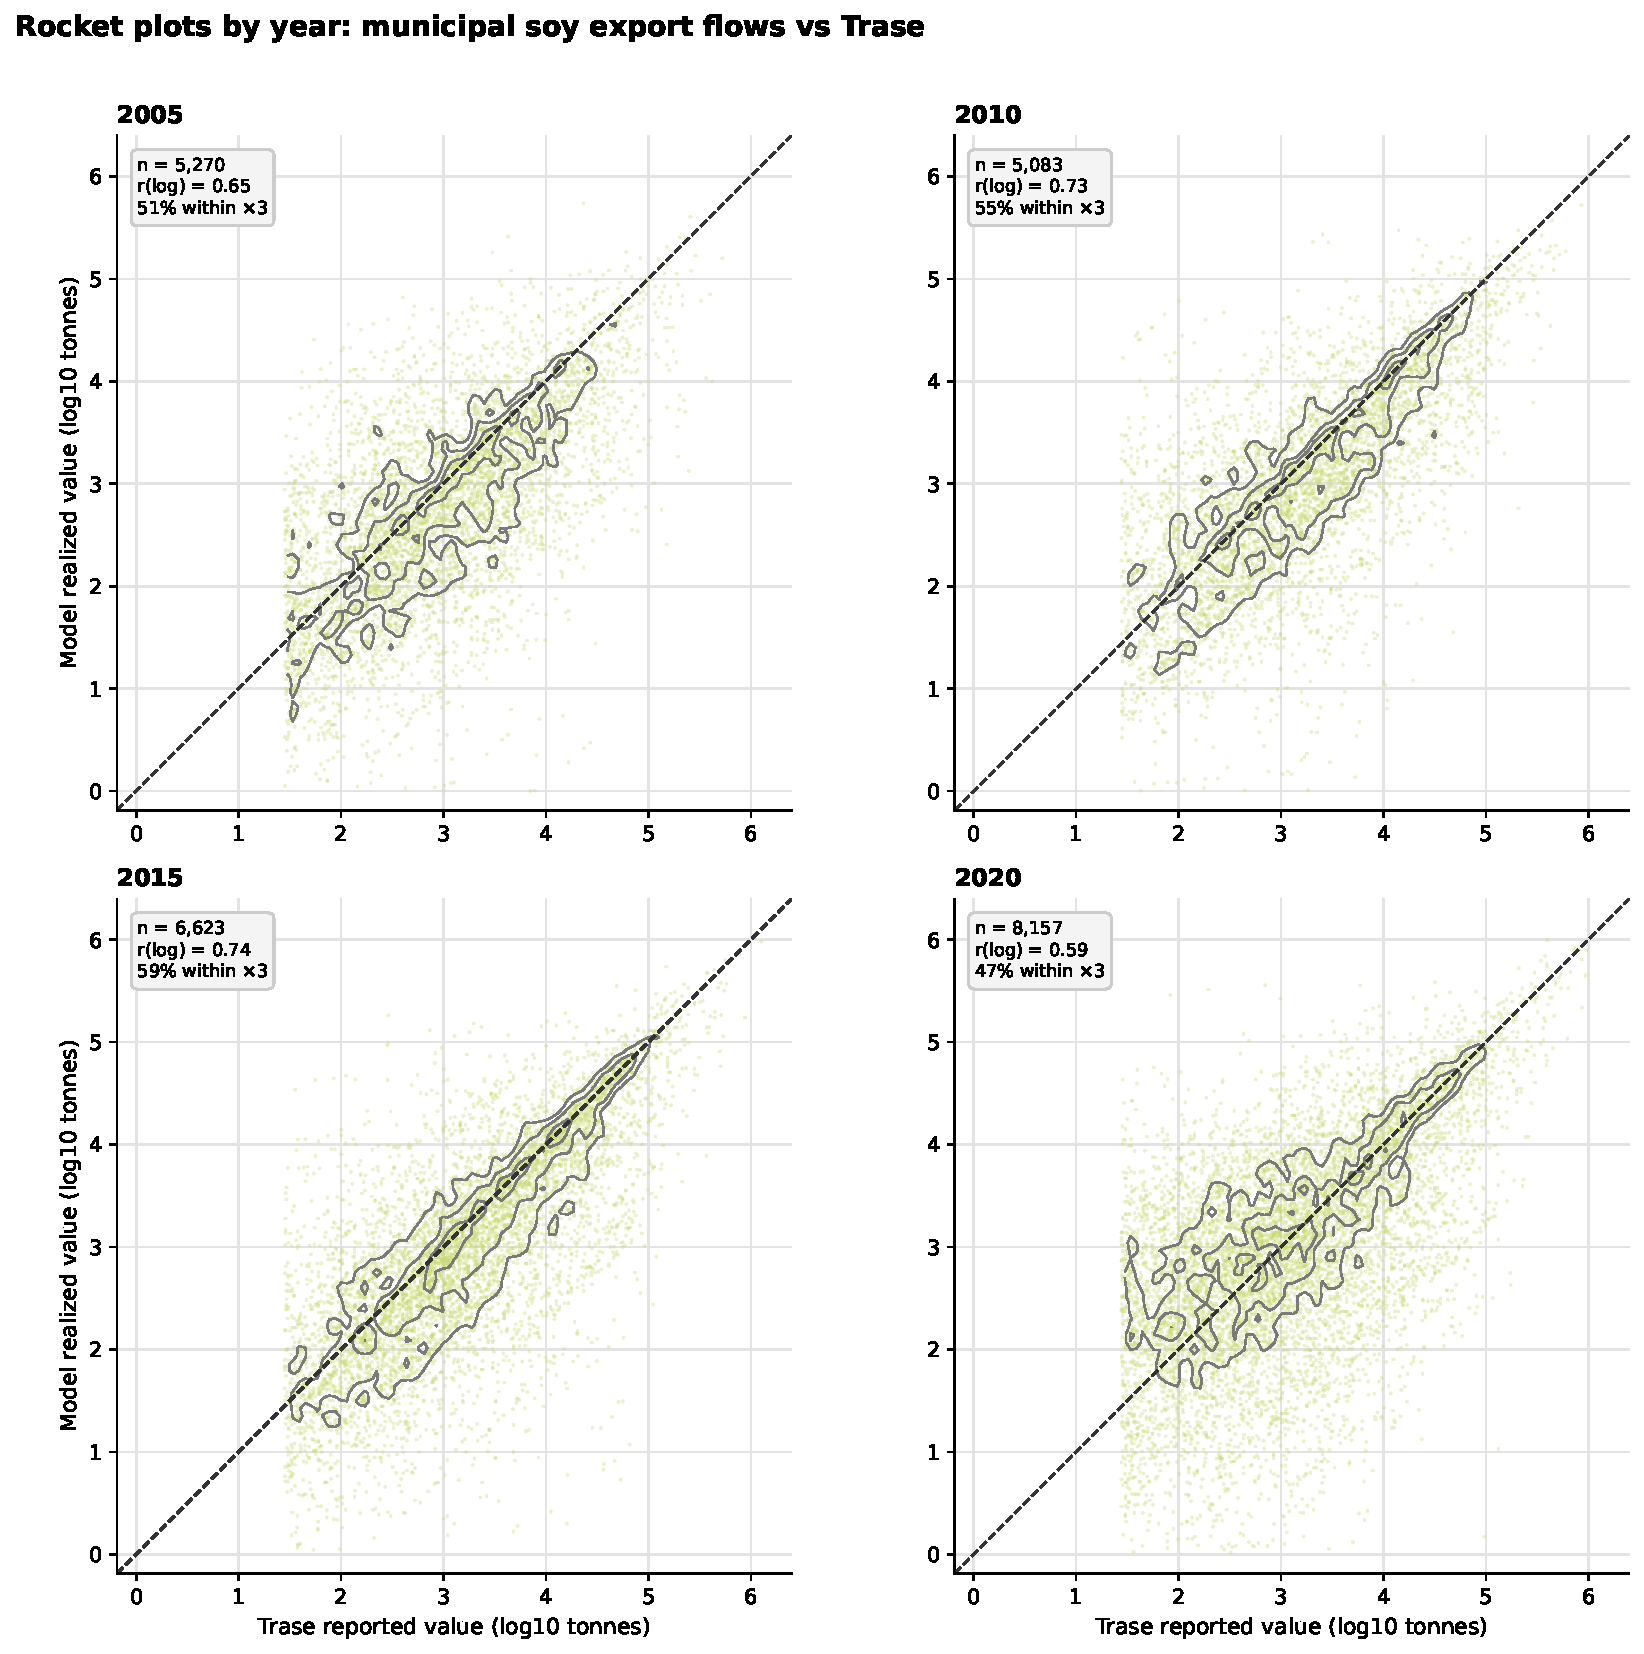
\includegraphics[width=0.94\textwidth]{figures/rocket_plot_years.pdf}
\caption{Agreement with the benchmark grows with flow size (``rocket
plots''). Every modelled municipality$\times$destination soy export flow is
plotted against the corresponding Trase flow (both $\log_{10}$ tonnes;
flows below 1\,t on either side are excluded) for four sample years, with
kernel-density contours and the 1:1 line (dashed); each panel reports the
number of matched flows, the log-scale Pearson correlation and the share of
flows agreeing within a factor of three. Large flows converge onto the 1:1
diagonal (the ``nose''), while small flows scatter (the ``plume''):
agreement rises systematically with volume, which motivates the volume
floor of the decision rule --- the tonnage that carries the footprint is
also the best-validated part of the flow
distribution.}\label{fig:rocket}
\end{figure}

\subsubsection{Uncertainty and sensitivity}\label{subsubsec:uncertainty}
% DEFERRED (2026-07-28), to run in one overnight batch:
%  (a) input-parameter OAT sensitivity -- perturb GLEAM feed intake (+-25%) and
%      the crush oil:cake split (+-2pp) to their bounds on 2013 (full pipeline),
%      report elasticities + a propagated ~90% interval on total / China / EU /
%      frontier footprints; one POF run to confirm it is second-order. Hooks are
%      in code (MC_FEED_MULT, MC_OILSHARE_DELTA, MC_POF_MULT, MC_CRUSHCAP_GAMMA);
%      driver: code/analysis/mc_sensitivity.R (TODO).
%  (b) productiveness-cap sensitivity -- re-run steps 17-20 at cap in
%      {0.99, 0.9999, 0.999999} for a representative year, plus a per-year table
%      of capped-column count / countries / item groups from uniform re-runs.
% The paragraph below states the structured sensitivity already in place.

The pipeline is deterministic, so uncertainty is characterized by structured
sensitivity rather than stochastic intervals, along four axes. (i)~Spatial
allocation tolerance: all agreement metrics are recomputed under the five
neighbourhood-smoothing schemes of Section~\ref{subsubsec:metrics}.
(ii)~Reference bracketing: every reported comparison places the model
between the downscaling baseline and the shipment-based
Trase benchmark, quantifying the value added by the supply-chain
structure. (iii)~Structural choices: the two admissible treatments
of net stock withdrawals (use-side proportional versus supply-side) are both
implemented and were compared on a test year; the supply-side treatment is
reported because it reflects the balance identity (a drawdown is a source of
current-year supply) and alone keeps all municipal uses non-negative
(Section~\ref{subsubsec:domuse}). (iv)~Backend vintage: the v1.1/v2 seam is
quantified by running the 2010--2013 overlap years through both chains
(Section~\ref{subsubsec:backend}); the $-6$ to $-8\%$ level difference and
$\geq$0.988 cross-country correlation of the clean overlap years bound the
vintage effect on pre-2010 results.
Agreement with the benchmark rises strongly with flow size, so the largest
flows, which carry most of the footprint, are also the best validated; results
for individual small-volume destinations (below the $\sim$$10^3$\,t floor of
Section~\ref{subsubsec:volcorr}) should be read with caution.

Finally, the proportional-mixing assumption of the trade-linkage inversion
(Section~\ref{subsubsec:reexport}) is probed by an origin-exclusion
counterfactual for the EU, where segregated and certified sourcing is
strongest. Setting the EU's Amazon-biome soy sourcing to zero --- a
perfect Amazon Soy Moratorium --- and redistributing that footprint across
the EU's remaining origins reallocates on average 0.9\,Mha\,yr$^{-1}$
(2010--2015) and moves the EU frontier-origin share from 28.8\% to between
16\% (displaced pro-rata to all non-Amazon origins) and 28.8\% (displaced
into the Cerrado frontier, which the moratorium does not cover); the
all-destination footprint is unchanged, as this only redistributes within
the EU consumption column. The bias is thus bounded and, notably, runs
counter to the deforestation narrative: the model already attributes a
higher Amazon-biome share to the EU (mean 14.8\%) than to China (9.4\%),
so correcting toward observed EU segregation would lower, not raise, the
EU's frontier footprint.

% ==================================================================
\subsection{Software}\label{subsec:software}
% ==================================================================
The pipeline is implemented in R (4.5; \texttt{data.table}, \texttt{dplyr},
\texttt{Matrix}, \texttt{sf}, \texttt{transport}) with figures and
web-map tooling in Python (3.14; \texttt{pandas}, \texttt{matplotlib},
\texttt{geopandas}). The reported results have no proprietary software
dependency; only the experimental multimodal-transport variant (not used
here) requires a GAMS licence.
